\documentclass[aps,twocolumn,secnumarabic,balancelastpage,amsmath,amssymb,nofootinbib]{revtex4}
% \documentclass[aps,twocolumn,secnumarabic,balancelastpage,amsmath,amssymb,nofootinbib]{revtex4}

% Documentclass Options

% nobalancelastpage doesn't attempt to equalize the lengths of the two columns
% on the last page as might be desired in a journal where articles follow one
% another closely
% amsmath and amssymb are necessary for the subequations environment among
% others secnumarabic identifies sections by number to aid electronic review
% and commentary. nofootinbib forces footnotes to occur on the page where they
% are first referenced and not in the bibliography

% \usepackage{lgrind}        % convert program listings to a form includable in a LaTeX document
\usepackage{chapterbib}    % allows a bibliography for each chapter (each labguide has it's own)
\usepackage{color}         % produces boxes or entire pages with colored backgrounds
\usepackage{graphics}      % standard graphics specifications
\usepackage[pdftex]{graphicx}      % alternative graphics specifications
\usepackage{longtable}     % helps with long table options
\usepackage{epsf}          % old package handles encapsulated post script issues
\usepackage{bm}            % special 'bold-math' package
\usepackage{tikz}
\usepackage{asymptote}     % For typesetting of mathematical illustrations
\usepackage{subfigure}

% \usepackage{thumbpdf}

\usepackage[colorlinks=true]{hyperref}  % this package should be added after all others
% use as follows: \url{http://web.mit.edu/8.13}
\newcommand{\drelectron}[1]{\node at #1 [circle, draw, inner sep=0pt, minimum size=1pt] {\_}}
\newcommand{\ud}{\mathrm{d}}
\newcommand{\ue}{\mathrm{e}}
\newcommand{\ui}{\mathrm{i}}
\newcommand{\res}{\mathrm{Res}}
\newcommand{\Tr}{\mathrm{Tr}}
\newcommand{\dsum}{\displaystyle\sum}
\newcommand{\dprod}{\displaystyle\prod}
\newcommand{\dlim}{\displaystyle\lim}
\newcommand{\dint}{\displaystyle\int}
\newcommand{\fsno}[1]{{\!\not\!{#1}}}
\newcommand{\eqar}[1]
{
  \begin{align*}
    #1
  \end{align*}
}
\newcommand{\texp}[2]{\ensuremath{{#1}\times10^{#2}}}
\newcommand{\dexp}[2]{\ensuremath{{#1}\cdot10^{#2}}}
\newcommand{\eval}[2]{{\left.{#1}\right|_{#2}}}
\newcommand{\paren}[1]{{\left({#1}\right)}}
\newcommand{\lparen}[1]{{\left({#1}\right.}}
\newcommand{\rparen}[1]{{\left.{#1}\right)}}
\newcommand{\abs}[1]{{\left|{#1}\right|}}
\newcommand{\sqr}[1]{{\left[{#1}\right]}}
\newcommand{\crly}[1]{{\left\{{#1}\right\}}}
\newcommand{\angl}[1]{{\left\langle{#1}\right\rangle}}
\newcommand{\tpdiff}[4][{}]{{\paren{\frac{\partial^{#1} {#2}}{\partial {#3}{}^{#1}}}_{#4}}}
\newcommand{\tpsdiff}[4][{}]{{\paren{\frac{\partial^{#1}}{\partial {#3}{}^{#1}}{#2}}_{#4}}}
\newcommand{\pdiff}[3][{}]{{\frac{\partial^{#1} {#2}}{\partial {#3}{}^{#1}}}}
\newcommand{\diff}[3][{}]{{\frac{\ud^{#1} {#2}}{\ud {#3}{}^{#1}}}}
\newcommand{\psdiff}[3][{}]{{\frac{\partial^{#1}}{\partial {#3}{}^{#1}} {#2}}}
\newcommand{\sdiff}[3][{}]{{\frac{\ud^{#1}}{\ud {#3}{}^{#1}} {#2}}}
\newcommand{\tpddiff}[4][{}]{{\left(\dfrac{\partial^{#1} {#2}}{\partial {#3}{}^{#1}}\right)_{#4}}}
\newcommand{\tpsddiff}[4][{}]{{\paren{\dfrac{\partial^{#1}}{\partial {#3}{}^{#1}}{#2}}_{#4}}}
\newcommand{\pddiff}[3][{}]{{\dfrac{\partial^{#1} {#2}}{\partial {#3}{}^{#1}}}}
\newcommand{\ddiff}[3][{}]{{\dfrac{\ud^{#1} {#2}}{\ud {#3}{}^{#1}}}}
\newcommand{\psddiff}[3][{}]{{\frac{\partial^{#1}}{\partial{}^{#1} {#3}} {#2}}}
\newcommand{\sddiff}[3][{}]{{\frac{\ud^{#1}}{\ud {#3}{}^{#1}} {#2}}}

\begin{document}
\tikzstyle{every picture}+=[remember picture]
\title{Optical Pumping of Rubidium Atoms in the Magnetic Field.}
\author{Yichao Yu}
\email{yuyichao@mit.edu}
\homepage{http://yyc-arch.org/}
\date{\today}
\affiliation{MIT Department of Physics}

\begin{abstract}
  The optical pumping is a technique that uses light to obtain non-thermal energy level distribution. It is important for atomic physics for state preparation and maintaining and is used in some standard laser cooling and trapping techniques. In this experiment, we studied the optical pumping between Zeeman levels in a magnetic field of rubidium atoms causing by a polaried light. We were able to measure some steady state properties like Landr\'e $g$-factors, abundance and ambient magnetic field as well as observe the transient state and measure the pumping rate and Rabi frequency.
\end{abstract}

\maketitle
%%%%%%%%%%%%%%%%%%%%%%%%%%%%%%%%%%%%%%%%%%%%%%%%%%%%%%%%%%%%%%%%%%
\section*{Introduction}
At thermal equilibrium, the population of energy levels of atoms is given by the Maxwell-Boltzmann distribution,
\[ \frac{n_1}{n_2}=\exp\paren{\frac{E_2-E_1}{k_BT}} \]

In the case of rubidium atoms at around room temperature ($300K$), the hyperfine splitting (around $20\mu eV$) and the Zeeman splitting in a weak ($<1Gs$) magnetic field (around $1neV$) is several orders of magnetude smaller than the thermal energy scale ($k_BT\approx20meV$) and therefore have equal occupation numbers in the thermal equilibrium. Optical pumping, however, can be used to break this equilibrium and ``pump'' almost all the atoms into a single Zeeman level using a circularly polarized light. The technique is very important and useful in atomic physics experiment either to prepare a starting state or to keep atoms in a certain state. It is also used in some standard laser cooling and trapping techniques like Zeeman slower and magnetic trap.

In our experiment, we studied the optical pumping of both ${}^{85}Rb$ and ${}^{87}Rb$ atoms using a rubidium lamp and a rubidium vapor cell at around $320K$. By changing the magnetic field and applying a radio frequency signal, we were able to measure the condition when the pumping happens or is destroyed as well as the transient state of the process.

\section{Theory.}
\subsection{Optical pumping between Zeeman levels using circularly polarized light.}
When placing atoms in a magnetic field, the energy level with


The recoil velocity and the Doppler shift caused by that are given by,
\eqar{
  v_{recoil}=&\frac{E}{2mc}\\
  \frac{\Delta E_{recoil}}{E}=&\frac{E}{2mc^2}
}
where $E$ is the original radiation energy, and $m$ is the mass of the nucleus. For the $14.4keV$ radiation used in this experiment and free atom in the gas, the relative recoil shift is $\dexp{2.8}{-7}$, $5$ orders of magnitude greater than the relative natural linewidth of the radiation $10^{-12}$. In order to elimiate the recoil effect, M\"{o}ssbauer embed the atom into a solid and therefore increase the mass in the denominator to an effective mass equal the the mass of the whole solid. Since the whole solid is about $10^{20}$ times heavier than the nucleus, the recoil shift is negligible.

By moving the source at a speed of the order $1cm\cdot s^{-1}$ under control, we are able to scan the energy of the $\gamma$-ray by $10^{10}-10^{11}$ and measure the absorption spectrum of the target material precisely in this small energy range.

\subsection{Shift and Splitting of energy levels.}
In this experiment, we are looking for several effects that can either shift or split the energy levels of a ${}^{57}Fe$ nucleus.

\subsubsection{Isomer shift}
This effect is caused by the non-zero electron density at the nucleus. Since the radius of the excited and ground state of the nucleus are slightly different, the energy shifts are also different for the two states and therefore also shift the energy of the radiation. The energy shift is given by,
\[\delta = C\delta R\abs{\psi(0)}^2\]
where $\delta R$ is the difference of the two radius, $\abs{\psi(0)}^2$ is the electron density at the nucleus, and $C$ is a constant. Since the isomer shift exists for all samples, what we are going to observe in the experiment is a relative difference between the shift for different sample.
\subsubsection{Zeeman effect}
\begin{figure}
  \includegraphics[width=8cm]{../share/zeeman.png}
  \caption{Zeeman effect.}
  \label{zeeman}
\end{figure}

The excited state of the ${}^{57}Fe$ nucleus has a total angular momentum $I=\dfrac32$ and the ground state has a total angular momentum $I=\dfrac12$. Therefore, when there is a magnetic field at the nucleus generated by other electrons and atoms in the sample, the zeeman effect will split the excited and the ground states into $4$ and $2$ different energy levels respectively generating $\gamma$ radiation of $6$ possible energies as shown in figure \ref{zeeman}.

The splitting and the energy correction of each levels are given by,
\eqar{
  \Delta E_I=&g_I\mu_NB\\
  E_I=&g_Im_I\mu_NB
}
where $g_I$ is the $g$-factor, $\mu_N$ is the nuclear magneton, $m_I$ is the angular momentum projection quantum number, and $B$ is the magnetic field.

\subsubsection{Quadrapole Splitting}
\begin{figure}
  \includegraphics[width=8cm]{../share/quad.png}
  \caption{Quadrapole Splitting.}
  \label{quad}
\end{figure}

This effect is caused by the interaction between nuclear quadrapole moment and the inhomogeneity of the electric field. This correction to the energy levels is given by,
\[\Delta E_{quad}=\frac{qe^2Q}{4I(2I-1)}\sqr{3m_I^2-I(I+1)}\]
where $q$ is the guadiant of the field, $Q$ the quadrapole moment. For the $I=\dfrac12$ ground state $\Delta E_{quad}=0$, whereas for the $I=\dfrac32$ excited state (Figure \ref{quad}),
\eqar{
  \Delta E_{quad}=\left\{\begin{array}{ll}
      \dfrac{qe^2Q}{4}&m_I=\pm\dfrac12\\
      -\dfrac{qe^2Q}{4}&m_I=\pm\dfrac32
    \end{array}
  \right.
}
\subsubsection{Temperature shift}
This is a small effect caused by the relativistic time dilation caused by the random heat motion of the nucleus. The shift is given by,
\[\frac{\delta}{E}=\frac{\angl{v^2}}{2c^2}=\frac{\angl{E_k}}{mc^2}\]
where $\angl{v^2}$ is the averge speed square and $\angl{E_k}$ is the average kinetic energy of the nucleus.

\subsubsection{Combination of multiple effects}
Multiple effects can exist in the same sample and at most $6$ absorption peaks can be observed. The energy shifts of these peaks are (temperature effect is ignored since it is small compare to other effects and will not change unless the temperature of the sample changes dramatically),
\eqar{
  \Delta E_1=&\varepsilon-\frac\delta2-\frac32\Delta_1-\frac12\Delta_0\\
  \Delta E_2=&\varepsilon+\frac\delta2-\frac12\Delta_1-\frac12\Delta_0\\
  \Delta E_3=&\varepsilon+\frac\delta2+\frac12\Delta_1-\frac12\Delta_0\\
  \Delta E_4=&\varepsilon+\frac\delta2-\frac12\Delta_1+\frac12\Delta_0\\
  \Delta E_5=&\varepsilon+\frac\delta2+\frac12\Delta_1+\frac12\Delta_0\\
  \Delta E_6=&\varepsilon-\frac\delta2+\frac32\Delta_1+\frac12\Delta_0
}
where $\varepsilon$ is the isomer shift, $\delta$ is the quadrapole splitting, $\Delta_1$ is the Zeeman splitting for the excited state and $\Delta_0$ is the Zeeman splitting for the ground state.

\section{Apparatus and calibration}
\subsection{Apparatus}
\begin{figure}
  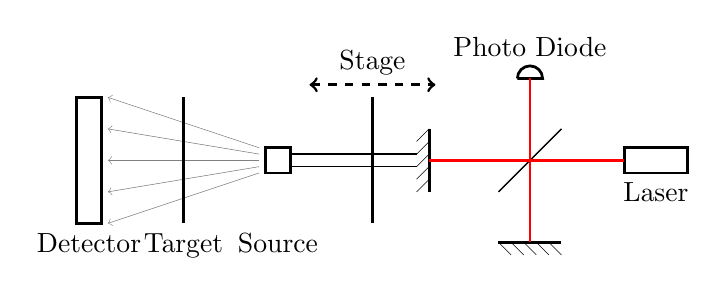
\begin{tikzpicture}[scale=.8]
    \path (2, 0) node[below] {Source};
    \draw[line width=.5] (3.5, .9) -- (2.2, .9);
    \draw[line width=.5] (2.2, 1.1) -- (3.5, 1.1);
    \draw[line width=1] (3.5, 0) -- (3.5, 2);
    \draw[line width=1] (2.2, 0.8) -- (2.2, 1.2) -- (1.8, 1.2) -- (1.8, 0.8) -- cycle;
    \draw[<->, dashed, black, line width=1] (2.5, 2.2) -- (4.5, 2.2);
    \path (3.5, 2.2) node[above] {Stage};
    \draw[line width=.5] (3.5, .9) -- (4.2, .9);
    \draw[line width=.5] (4.2, 1.1) -- (3.5, 1.1);

    \draw[line width=.2, ->, gray] (1.7, 1.2) -- (-0.7, 2);
    \draw[line width=.2, ->, gray] (1.7, 1.1) -- (-0.7, 1.5);
    \draw[line width=.2, ->, gray] (1.7, 1.0) -- (-0.7, 1);
    \draw[line width=.2, ->, gray] (1.7, .9) -- (-0.7, .5);
    \draw[line width=.2, ->, gray] (1.7, .8) -- (-0.7, 0);

    \draw[line width=1] (4.4, 1.5) -- (4.4, 0.5);
    \draw[line width=.2] (4.4, 1.5) -- ++(-.2, -.2);
    \draw[line width=.2] (4.4, 1.3) -- ++(-.2, -.2);
    \draw[line width=.2] (4.4, 1.1) -- ++(-.2, -.2);
    \draw[line width=.2] (4.4, 0.9) -- ++(-.2, -.2);
    \draw[line width=.2] (4.4, 0.7) -- ++(-.2, -.2);

    \draw[line width=.5] (5.5, 0.5) -- (6.5, 1.5);

    \draw[line width=1] (5.5, -.3) -- (6.5, -.3);
    \draw[line width=.2] (5.5, -.3) -- ++(.2, -.2);
    \draw[line width=.2] (5.7, -.3) -- ++(.2, -.2);
    \draw[line width=.2] (5.9, -.3) -- ++(.2, -.2);
    \draw[line width=.2] (6.1, -.3) -- ++(.2, -.2);
    \draw[line width=.2] (6.3, -.3) -- ++(.2, -.2);

    \draw[line width=1] (7.5, 1.2) -- (7.5, 0.8) -- (8.5, 0.8) -- (8.5, 1.2) -- cycle;
    \path (8, 0.8) node[below] {Laser};

    \draw[line width=1] (5.8, 2.3) -- (6.2, 2.3) arc (0:180:.2);
    \path (6, 2.5) node[above] {Photo Diode};

    \draw[line width=1, red] (4.4, 1) -- (7.5, 1);
    \draw[line width=1, red] (6, 2.3) -- (6, -.3);

    \path (-1, 0) node[below] {Detector};
    \draw[line width=1] (-1.2, 0) -- (-1.2, 2) -- (-.8, 2) -- (-.8, 0) -- cycle;

    \path (0.5, 0) node[below] {Target};
    \draw[line width=1] (0.5, 0) -- (0.5, 2);
  \end{tikzpicture}
  \caption{Apparatus.}
  \label{apparatus}
\end{figure}

Figure \ref{apparatus} is a schematics of the apparatus used in this experiment. The source is attached on a stage that can be moved back and forth in cycles under control of the computer. A detector will measure the counting rate of radiation after absorbed by the target sample as a function of time in each scanning cycle and also send the data back to the computer. The source used in the experiment is ${}^{57}Co$, which will first decay by a $K$ capture to a ${}^{57}Fe$ nucleus. After another $\gamma$ decay, the nucleus finally go to its ground state by emitting a $\gamma$-ray photon at the energy $14.4keV$, which is the $\gamma$-ray we are using in the experiment.

\subsection{Calibration of velocity using Michelson interferometer.}
A Michelson interferometer with one mirror attached to the moving stage is used to calibrate the moving velocity of the stage (right half of figure \ref{apparatus}). By measuring the power using the photo diode, the speed of the stage is,
\eqar{
  \abs{v}=&2f\lambda
}
where $f$ is the frequency of the laser power and $\lambda=632.8nm$ is the wavelength of the $He$-$Ne$ laser used in the interferometer.
\begin{figure}
  \includegraphics[width=8cm]{../pos_cal/res_v_raw.png}
  \caption{Measurement of stage speed in each cycle. Each channel number in the horizontal axis corresponds to a certain time point in each scanning cycle.}
  \label{v_raw}
\end{figure}
\begin{figure}
  \includegraphics[width=8cm]{../pos_cal/res_v_fit.png}
  \caption{Calibration fitting of velocity.}
  \label{v_fit}
\end{figure}

Figure \ref{v_raw} shows the relation between the speed of the stage and the time in each cycle (which is shown as channel numbers). After removing the first part where the velocity is changing rapidly and flip the sign for the region where the velocity is negetive, the calibration line was obtained by fitting a straight line to the data, as shown in figure \ref{v_fit}.

\section{Measurement of different samples}
\subsection{$Fe$, $Fe_2O_3$, $FeSO_4$ and $Fe_2(SO_4)_3$ samples}
\begin{figure}
  \subfigure[$Fe$]{
    \includegraphics[width=8cm]{../pos_cal/02-14-6_2_raw.png}
    \label{fe_raw}
  }
  \subfigure[$FeSO_4$]{
    \includegraphics[width=8cm]{../FeSO4_Fe2SO4_3/02-19-FeSO4_raw.png}
    \label{feso4_raw}
  }
  \caption{Measured absorption spectrum of \subref{fe_raw} $Fe$ and \subref{feso4_raw} $FeSO_4$ samples. The light blue curves are the original data, the dark blue curves are the data after being smoothed. The vertical lines shows the position of peaks and the horizontal lines is an estimation of the total radiation level (without absorption of the target).}
  \label{samples_raw}
\end{figure}

Each of the $Fe$, $Fe_2O_3$, $FeSO_4$ and $Fe_2(SO_4)_3$ samples has one or more effects among isomer shift, zeeman effect and quadrapole splitting. By determining the position of peaks in the measured spectrum (figure \ref{samples_raw}) and using the expression of the correction for each peaks given in section 1.2.5, we can calculate the correction caused by different effects on each samples. The results of the calculation as well as the accepted value for each energy corrections are shown in table \ref{res_table}. All of our measurement agree with the accepted value very well and the deviations are all not greater than $1.5\sigma$.

\begin{table}
  \begin{tabular}{|c|c|c|c|c|}
    \hline
    Sample&Effect&Measured&Accepted&Deviation\\\hline
    $Fe$\cite{data3}&$\Delta_0$&$188.2(1.3)$&$188.38(38)$&$0.1\sigma$\\\cline{2-5}
    &$\Delta_1$&$107.4(1.3)$&$107.83(24)$&$0.3\sigma$\\\hline
    $Fe_2O_3$\cite{data1}\cite{data2}&$\Delta_0$&$296.8(1.7)$&$293.5(2.4)$&$0.8\sigma$\\\cline{2-5}
    &$\Delta_1$&$171.8(1.7)$&$165.7(2.4)$&$1.5\sigma$\\\cline{2-5}
    &$\delta$&$9.4(1.6)$&$11.5(1.4)$&$0.7\sigma$\\\cline{2-5}
    &$\varepsilon$&$39(18)$&$22.6(1.4)$&$0.8\sigma$\\\hline
    $FeSO_4$\cite{data1}&$\delta$&$156.2(0.2)$&$153.7(2.4)$&$0.96\sigma$\\\cline{2-5}
    &$\varepsilon$&$59(14)$&$67.2(2.4)$&$0.5\sigma$\\\hline
    $Fe_2(SO_4)_3$\cite{data1}&$\varepsilon$&$29(16)$&$31.2(2.4)$&$0.1\sigma$\\\hline
  \end{tabular}
  \caption{Results for different energy level corrections on different samples. $\Delta_0$ and $\Delta_1$ are the Zeeman splitting of the groud state and the excited state respectively. $\delta$ is the quadrapole splitting and $\varepsilon$ is the isomer shift. (Unit of energy $10^{-9}eV$).}
  \label{res_table}
\end{table}

\subsection{Measurement of natural line width using $Na_4Fe(CN)_6$ samples.}
\begin{figure}
  \includegraphics[width=8cm]{../share/line_width.png}
  \caption{FWHM ($2\Gamma$) of absorption peaks for different amount of $Na_4Fe(CN)_6$ power samples.}
  \label{line_width}
\end{figure}
The line width (FWHM) of the peaks for different amount of $Na_4Fe(CN)_6$ power samples are shown in figure \ref{line_width}. By fitting a straight line to the data, the natural line width (FWHM) of the absorption at thin sample limit we measured in the experiment is $\dexp{1.60(30)}{-8}eV$. Comparing to the accepted value of the line width $\dexp{9.4}{-9}eV$, the value we measured is $2.2\sigma$ larger. This different can caused by a variety of broadening effect in our measurement including a finite temperature and the velocity uncertainty of the stage.

\subsection{Measurement of temperature shift using stainless steel sample.}
\begin{figure}
  \subfigure[$21^{\circ}C$]{
    \includegraphics[width=8cm]{../temp/02-25-21c_raw.png}
    \label{temp_21_raw}
  }
  \subfigure[$130^{\circ}C$]{
    \includegraphics[width=8cm]{../temp/02-26-130c_raw.png}
    \label{temp_130_raw}
  }
  \caption{Measured absorption spectrum of stainless steel sample at \subref{temp_21_raw} $21^{\circ}C$ and \subref{temp_130_raw} $130^{\circ}C$. The red verticle lines show the position of the peak and the green verticle line shows the uncertainty of the position. The uncertainty is magnified by a factor of $4$ in order to be seen clearly on the plot.}
  \label{temp_raw}
\end{figure}
In order to measure the temperature shift caused by relativistic time dilation, we measured the stainless steel sample (which has no splitting effect) at $21(1)^{\circ}C$ and $130(5)^{\circ}C$. From the results shown in figure \ref{temp_raw} (The uncertainty is magnified by a factor of $4$ in order to be seen clearly on the plot), we found a relative energy shift in the $\gamma$-ray spectrum of $1.86(69)\cdot 10^{-13}$. Using a classic model and a Debye model of crystal vibration, we can calculate the expected value of the energy shift using the expression of average kinetic energy from different model,
\eqar{
  E_{classic}=&\frac32k_BT\\
  E_{Debye}=&\frac{9k_BT^4}{10\Theta_D^3}D_3\paren{\frac{T}{\Theta_D}}
}
where $\Theta_D\approx470$ is the Debye temperature estimated using that of Iron. A comparison of the average kinetic energy of nucleus calculated using different methods is shown in table \ref{temp_model}. The value we have measured is within $1\sigma$ of the expected value from Debye model and it is also not far from the result of classic model since we are close to the high temperature limit.

\begin{table}
  \begin{tabular}{|c|c|}
    \hline
    Model&$E_k$\\\hline
    Classic&$1.409(12)\cdot 10^{-2}eV$\\\hline
    Debye&$1.304(84)\cdot 10^{-2}eV$\\\hline
    (Measured)&$0.99(36)\cdot 10^{-2}eV$\\\hline
  \end{tabular}
  \caption{Average kinetic energy of nucleus calculated using different methods.}
  \label{temp_model}
\end{table}

\section{Conclusion}
In this experiment, we finished our main goal of measuring the spectrum of ${}^{57}Fe$ nucleus $14.4keV$ $\gamma$-radiation using M\"{o}ssbauer effect. By measuring the spectrum, we determined the energy correction caused by different effects which agrees very well with the accepted value. The natural line width we have measured is larger than the accepted onebecause of some broadening effects and our measurement of temperature shift agrees with theoritical perdiction very well.

\bibliography{report}
\end{document}
